\documentclass[english,hidelinks, 11 pt, class=report,crop=false]{standalone}
\usepackage[T1]{fontenc}
%\usepackage[utf8]{inputenc}
\usepackage{lmodern} % load a font with all the characters
\usepackage{geometry}
\geometry{verbose,paperwidth=16.1 cm, paperheight=24 cm, inner=2.3cm, outer=1.8 cm, bmargin=2cm, tmargin=1.8cm}
\setlength{\parindent}{0bp}
\usepackage{import}
\usepackage[subpreambles=false]{standalone}
\usepackage{amsmath}
\usepackage{amssymb}
\usepackage{esint}
\usepackage{babel}
\usepackage{tabu}
\makeatother
\makeatletter

\usepackage{titlesec}
\usepackage{ragged2e}
\RaggedRight
\raggedbottom
\frenchspacing

\usepackage{graphicx}
\usepackage{float}
\usepackage{subfig}
\usepackage{placeins}
\usepackage{cancel}
\usepackage{framed}
\usepackage{wrapfig}
\usepackage[subfigure]{tocloft}
\usepackage[font=footnotesize,labelfont=sl]{caption} % Figure caption
\usepackage{bm}
\usepackage[dvipsnames, table]{xcolor}
\definecolor{shadecolor}{rgb}{0.105469, 0.613281, 1}
\colorlet{shadecolor}{Emerald!15} 
\usepackage{icomma}
\makeatother
\usepackage[many]{tcolorbox}
\usepackage{multicol}
\usepackage{stackengine}

\usepackage{esvect} %For vectors with capital letters

% For tabular
\usepackage{array}
\usepackage{multirow}
\usepackage{longtable} %breakable table

% Ligningsreferanser
\usepackage{mathtools} % for mathclap
%\mathtoolsset{showonlyrefs}

% sections without numbering in toc
\newcommand\tsec[1]{\phantomsection \addcontentsline{toc}{section}{#1}
	\section*{#1}}

% index
\usepackage{imakeidx}
\makeindex[title=Indeks]

%Footnote:
\usepackage[bottom, hang, flushmargin]{footmisc}
\usepackage{perpage} 
\MakePerPage{footnote}
\addtolength{\footnotesep}{2mm}
\renewcommand{\thefootnote}{\arabic{footnote}}
\renewcommand\footnoterule{\rule{\linewidth}{0.4pt}}
\renewcommand{\thempfootnote}{\arabic{mpfootnote}}

%colors
\definecolor{c1}{cmyk}{0,0.5,1,0}
\definecolor{c2}{cmyk}{1,0.25,1,0}
\definecolor{n3}{cmyk}{1,0.,1,0}
\definecolor{neg}{cmyk}{1,0.,0.,0}


\newcommand{\nreq}[1]{
\begin{equation}
	#1
\end{equation}
}


% Equation comments
\newcommand{\cm}[1]{\llap{\color{blue} #1}}


\usepackage[inline]{enumitem}
\newcounter{rg}
\numberwithin{rg}{chapter}


\newcommand{\reg}[2][]{\begin{tcolorbox}[boxrule=0.3 mm,arc=0mm,colback=blue!3] {\refstepcounter{rg}\phantomsection \large \textbf{\therg \;#1} \vspace{5 pt}}\newline #2  \end{tcolorbox}\vspace{-5pt}}
\newcommand{\regdef}[2][]{\begin{tcolorbox}[boxrule=0.3 mm,arc=0mm,colback=blue!3] {\refstepcounter{rg}\phantomsection \large \textbf{\therg \;#1} \vspace{5 pt}}\newline #2  \end{tcolorbox}\vspace{-5pt}}
\newcommand{\words}[1]{\begin{tcolorbox}[boxrule=0.3 mm,arc=0mm,colback=teal!3] #1  \end{tcolorbox}\vspace{-5pt}}

\newcommand\alg[1]{\begin{align*} #1 \end{align*}}

\newcommand\eks[2][]{\begin{tcolorbox}[boxrule=0.3 mm,arc=0mm,enhanced jigsaw,breakable,colback=green!3] {\large \textbf{\ekstitle #1} \vspace{5 pt}\\} #2 \end{tcolorbox}\vspace{-5pt} }

\newcommand{\st}[1]{\begin{tcolorbox}[boxrule=0.0 mm,arc=0mm,enhanced jigsaw,breakable,colback=yellow!12]{ #1} \end{tcolorbox}}

\newcommand{\spr}[1]{\begin{tcolorbox}[boxrule=0.3 mm,arc=0mm,enhanced jigsaw,breakable,colback=yellow!7] {\large \textbf{\sprtitle} \vspace{5 pt}\\} #1 \end{tcolorbox}\vspace{-5pt} }

\newcommand{\sym}[1]{\colorbox{blue!15}{#1}}

\newcommand{\info}[2]{\begin{tcolorbox}[boxrule=0.3 mm,arc=0mm,enhanced jigsaw,breakable,colback=cyan!6] {\large \textbf{#1} \vspace{5 pt}\\} #2 \end{tcolorbox}\vspace{-5pt} }

\newcommand\algv[1]{\vspace{-11 pt}\begin{align*} #1 \end{align*}}

\newcommand{\regv}{\vspace{5pt}}
\newcommand{\mer}{\textsl{\note}: }
\newcommand{\mers}[1]{{\footnotesize \mer #1}}
\newcommand\vsk{\vspace{11pt}}
\newcommand{\tbs}{\vspace{5pt}}
\newcommand\vs{\vspace{-11pt}}
\newcommand\vsb{\vspace{-16pt}}
\newcommand\br{\\[5 pt]}
\newcommand{\figp}[1]{../fig/#1}
\newcommand\algvv[1]{\vs\vs\begin{align*} #1 \end{align*}}
\newcommand{\y}[1]{$ {#1} $}
\newcommand{\os}{\\[5 pt]}
\newcommand{\prbxl}[2]{
\parbox[l][][l]{#1\linewidth}{#2
	}}
\newcommand{\prbxr}[2]{\parbox[r][][l]{#1\linewidth}{
		\setlength{\abovedisplayskip}{5pt}
		\setlength{\belowdisplayskip}{5pt}	
		\setlength{\abovedisplayshortskip}{0pt}
		\setlength{\belowdisplayshortskip}{0pt} 
		\begin{shaded}
			\footnotesize	#2 \end{shaded}}}
\newcommand{\fgbxr}[2]{
	\parbox[r][][l]{#1\linewidth}{#2
}}		

\renewcommand{\cfttoctitlefont}{\Large\bfseries}
\setlength{\cftaftertoctitleskip}{0 pt}
\setlength{\cftbeforetoctitleskip}{0 pt}

\newcommand{\bs}{\\[3pt]}
\newcommand{\vn}{\\[6pt]}
\newcommand{\fig}[1]{\begin{figure}[H]
		\centering
		\includegraphics[]{\figp{#1}}
\end{figure}}

\newcommand{\figc}[2]{\begin{figure}
		\centering
		\includegraphics[]{\figp{#1}}
		\caption{#2}
\end{figure}}
\newcommand{\arc}[1]{{
		\setbox9=\hbox{#1}%
		\ooalign{\resizebox{\wd9}{\height}{\texttoptiebar{\phantom{A}}}\cr\textit{#1}}}}

\newcommand{\sectionbreak}{\clearpage} % New page on each section

\newcommand{\nn}[1]{
\begin{equation*}
	#1
\end{equation*}
}

\newcommand{\enh}[1]{\,\textrm{#1}}

%asin, atan, acos
\DeclareMathOperator{\atan}{atan}
\DeclareMathOperator{\acos}{acos}
\DeclareMathOperator{\asin}{asin}

% Comments % old cm, ggb cm is new
%\newcommand{\cm}[1]{\llap{\color{blue} #1}}

%%%

\newcommand\fork[2]{\begin{tcolorbox}[boxrule=0.3 mm,arc=0mm,enhanced jigsaw,breakable,colback=yellow!7] {\large \textbf{#1 (\expl)} \vspace{5 pt}\\} #2 \end{tcolorbox}\vspace{-5pt} }
 
%colors
\newcommand{\colr}[1]{{\color{red} #1}}
\newcommand{\colb}[1]{{\color{blue} #1}}
\newcommand{\colo}[1]{{\color{orange} #1}}
\newcommand{\colc}[1]{{\color{cyan} #1}}
\definecolor{projectgreen}{cmyk}{100,0,100,0}
\newcommand{\colg}[1]{{\color{projectgreen} #1}}

% Methods
\newcommand{\metode}[2]{
	\textsl{#1} \\[-8pt]
	\rule{#2}{0.75pt}
}

%Opg
\newcommand{\abc}[1]{
	\begin{enumerate}[label=\alph*),leftmargin=18pt]
		#1
	\end{enumerate}
}
\newcommand{\abcs}[2]{
	\begin{enumerate}[label=\alph*),start=#1,leftmargin=18pt]
		#2
	\end{enumerate}
}
\newcommand{\abcn}[1]{
	\begin{enumerate}[label=\arabic*),leftmargin=18pt]
		#1
	\end{enumerate}
}
\newcommand{\abch}[1]{
	\hspace{-2pt}	\begin{enumerate*}[label=\alph*), itemjoin=\hspace{1cm}]
		#1
	\end{enumerate*}
}
\newcommand{\abchs}[2]{
	\hspace{-2pt}	\begin{enumerate*}[label=\alph*), itemjoin=\hspace{1cm}, start=#1]
		#2
	\end{enumerate*}
}

% Exercises


\newcounter{opg}
\numberwithin{opg}{section}

\newcounter{grub}
\numberwithin{opg}{section}
\newcommand{\op}[1]{\vspace{15pt} \refstepcounter{opg}\large \textbf{\color{blue}\theopg} \vspace{2 pt} \label{#1} \\}
\newcommand{\eksop}[2]{\vspace{15pt} \refstepcounter{opg}\large \textbf{\color{blue}\theopg} (#1) \vspace{2 pt} \label{#2} \\}

\newcommand{\nes}{\stepcounter{section}
	\setcounter{opg}{0}}
\newcommand{\opr}[1]{\vspace{3pt}\textbf{\ref{#1}}}
\newcommand{\oeks}[1]{\begin{tcolorbox}[boxrule=0.3 mm,arc=0mm,colback=white]
		\textit{\ekstitle: } #1	  
\end{tcolorbox}}
\newcommand\opgeks[2][]{\begin{tcolorbox}[boxrule=0.1 mm,arc=0mm,enhanced jigsaw,breakable,colback=white] {\footnotesize \textbf{\ekstitle #1} \\} \footnotesize #2 \end{tcolorbox}\vspace{-5pt} }


% tag exercises
\newcommand{\tagop}[1]{ 
{\small \color{Gray} #1} \os
}

% License
\newcommand{\lic}{
This book is part of the \net{https://sindrsh.github.io/openmathbooks/}{OpenMathBooks} project. OpenMathBooks © 2022 by Sindre Sogge Heggen is licensed under CC BY-NC-SA 4.0. To view a copy of this license, visit \net{http://creativecommons.org/licenses/by-nc-sa/4.0/}{http://creativecommons.org/licenses/by-nc-sa/4.0/}}

%referances
\newcommand{\net}[2]{{\color{blue}\href{#1}{#2}}}
\newcommand{\hrs}[2]{\hyperref[#1]{\color{blue}#2 \ref*{#1}}}
\newcommand{\refunnbr}[2]{\hyperref[#1]{\color{blue}#2}}


\newcommand{\openmath}{\net{https://sindrsh.github.io/openmathbooks/}{OpenMathBooks}}
\newcommand{\am}{\net{https://sindrsh.github.io/FirstPrinciplesOfMath/}{AM1}}
\newcommand{\mb}{\net{https://sindrsh.github.io/FirstPrinciplesOfMath/}{MB}}
\newcommand{\tmen}{\net{https://sindrsh.github.io/FirstPrinciplesOfMath/}{TM1}}
\newcommand{\tmto}{\net{https://sindrsh.github.io/FirstPrinciplesOfMath/}{TM2}}
\newcommand{\amto}{\net{https://sindrsh.github.io/FirstPrinciplesOfMath/}{AM2}}
\newcommand{\eksbm}{
\footnotesize
Dette er opppgaver som har blitt gitt ved sentralt utformet eksamen i Norge. Oppgavene er laget av Utdanningsdirektoratet. Forkortelser i parantes viser til følgende:
\begin{center}
	\begin{tabular}{c|c}
		E & Eksempeloppgave \\
		V/H & Eksamen fra vårsemesteret/høstsemesteret\\
		G/1P/1T/R1/R2 & Fag  \\
		XX & År 20XX \\
		D1/D2 & Del 1/Del 2
	\end{tabular}
\end{center}
Tekst og innhold kan her være noe endret i forhold til originalen.
}

%Excel og GGB:

\newcommand{\g}[1]{\begin{center} {\tt #1} \end{center}}
\newcommand{\gv}[1]{\begin{center} \vspace{-11 pt} {\tt #1}  \end{center}}
\newcommand{\cmds}[2]{{\tt #1}\\
	#2}

% outline word
\newcommand{\outl}[1]{{\boldmath \color{teal}\textbf{#1}}}
%line to seperate examples
\newcommand{\linje}{\rule{\linewidth}{1pt} }


%Vedlegg
\newcounter{vedl}
\newcounter{vedleq}
\renewcommand\thevedl{\Alph{vedl}}	
\newcommand{\nreqvd}{\refstepcounter{vedleq}\tag{\thevedl \thevedleq}}

%%% Writing code

\usepackage{listings}


\definecolor{codegreen}{rgb}{0,0.6,0}
\definecolor{codegray}{rgb}{0.5,0.5,0.5}
\definecolor{codepurple}{rgb}{0.58,0,0.82}
\definecolor{backcolour}{rgb}{0.95,0.95,0.92}

\newcommand{\pymet}[1]{{\ttfamily\color{magenta} #1}}
\newcommand{\pytype}[1]{{\ttfamily\color{codepurple} #1}}

\lstdefinestyle{mystyle}{
	backgroundcolor=\color{backcolour},   
	commentstyle=\color{codegreen},
	keywordstyle=\color{magenta},
	numberstyle=\tiny\color{codegray},
	stringstyle=\color{codepurple},
	basicstyle=\ttfamily\footnotesize,
	breakatwhitespace=false,         
	breaklines=true,                 
	captionpos=b,                    
	keepspaces=true,                 
	numbers=left,                    
	numbersep=5pt,                  
	showspaces=false,                
	showstringspaces=false,
	showtabs=false,                  
	tabsize=2,
	inputencoding=utf8,
	extendedchars=true,
	literate= {
		{å}{{\aa}}1 
		{æ}{{\ae}}1 
		{ø}{{\o}}1
	}
}

\lstset{style=mystyle}

\newcommand{\python}[1]{
\begin{tcolorbox}[boxrule=0.3 mm,arc=0mm,colback=white]
\lstinputlisting[language=Python]{#1}
\end{tcolorbox}}
\newcommand{\pythonut}[2]{
\begin{tcolorbox}[boxrule=0.3 mm,arc=0mm,colback=white]
\small 
%\textbf{Kode}
\lstinputlisting[language=Python]{#1}	
\vspace{11pt}
\textbf{Utdata} \\ \ttfamily
#2
\end{tcolorbox}}
%%%

%page number
%\usepackage{fancyhdr}
%\pagestyle{fancy}
%\fancyhf{}
%\renewcommand{\headrule}{}
%\fancyhead[RO, LE]{\thepage}

\usepackage{datetime2}
%%\usepackage{sansmathfonts} for dyslexia-friendly math
\usepackage[]{hyperref}




\begin{document}
{\Large Eksamen R1 Våren 2024\hfill {\footnotesize Løsning fra \color{blue} \href{https://sindreheggen.wordpress.com/}{OpenMathBooks prosjektet}}}
\subsection*{Oppgave 1}	
Bruker produktregelen og kjerneregelen, og får at
\alg{
\left(4x^2\cdot \ln(3x)\right)' &= (4x^2)'\ln(3x)+4x^2(\ln (3x))' \\
&= 8x\ln(3x)+4x^2\frac{1}{3x}\cdot 3 \\
&= 4x(2\ln(3x)+1)
}

\subsection*{Oppgave 2}
Vi setter $ \ln x =u $, og får at
\[ u^2-u-6=0 \]
Da $ 2(-3)=-6 $ og $ 2+(-3)=-1 $, har vi at
\[ (u+2)(u-3)=0 \]
Dermed er 
\alg{
\ln x &= -2 &&\vee & \ln x &= 3 \\
x &= e^{-2} &&\vee & x &= e^3
}

\subsection*{Oppgave 3}
\algv{
\lim\limits_{x\to\infty}f(x)&= \lim\limits_{x\to\infty} e^{-\infty+1}\lim\limits_{x\to\infty} \frac{1}{e^\infty}=0 \vn
\lim\limits_{x\to\infty}f(x)&= \lim\limits_{x\to\infty} e^{-(-\infty)+1}\lim\limits_{x\to-\infty} e^\infty=\infty
}
Altså er det bare den øverste grensen som eksisterer.

\newpage
\subsection*{Oppgave 4}
\abc{
\item Hvis $ A $, $ B $ og $ C $ ligger på linje, er $ \vv{AB}\parallel \vv{AC} $. Vi har at
\alg{
	\vv{AB}&= [-1-3, -2-4] = -2[2, 3] \vn
	\vv{AC}&= [t, 2t-4]
}
Da forholdet mellom $ x $-koordinaten og $ y $-koordinaten til $ \vv{AB} $ er $ \frac{2}{3} $ har vi at
\alg{
	\frac{t}{2t-4}&=\frac{2}{3}\\
	3t &= 2(2t-4) \\
	t &= 8
}
\item $ \vv{AB} $ og $ \vv{AC} $ danner en rett vinkel hvis $ \vv{AB}\cdot\vv{AC}=0 $, som betyr at
\alg{
[2, 3]\cdot[t, 2t-4]&= 0 \\
2t+3(2t-4)&=0 \\
t &= \frac{1}{2}
}
}
\newpage
\subsection*{Oppgave 1}
\abc{
\item Det tar ca. 9 dager før 100 elever er smittet (rad 2).
\item Tidspunktet der flest blir smittet er der $ S'(t) $ har sitt maksimum, som er når $ t\approx 11 $ (rad 3). Flest blir altså smittet rundt dag 11, og da blir mellom 22 til 23 elever smittet per dag.
\item For $ t>0 $ er $ y=300 $ en horisontal asymptote til $ S $. Dette betyr at det aldri vil bli mer enn 300 smittede elever ved skolen.
}
\localfig{opg1}{0.3}

\subsection*{Oppgave 2}
\abc{
\item Påstanden er sann fordi hvis $ x>0 $ har vi at
\[ e^{k\ln x}=(e^{\ln x})^k=x^k \]
\item
\alg{
&\lim\limits_{x\to 2} (x^3-2)'=\lim\limits_{x\to 2} 3x^2 = 8 \vn
&\lim\limits_{x\to 2} (3x^2-4)' = \lim\limits_{x\to 2} 6x = 12
}
Skulle $ f $ vært deriverbar i $ x=2 $ måtte dei to uttrykkene over hatt lik grenseverdi, og det har de ikke. Påstanden er feil.
\item Hvis en funksjon $ f(x) $ er både minkende og voksende i en sammenhende definisjonsmengde, vil $ f $ anta lik verdi for minst to forskjellige verdier av $ x $, og kan da ikke ha en omvendt funksjon. I så fall er påstanden er feil. Hvis $ f $ derimot har delt forskrift, minkende på en delmengde og voksende på en annen delmengde, er påstanden sann.
}
\subsection*{Oppgave 3}
\abc{
\item Vi definerer $ r_a $ og $ r_b $ som henholdsvis $ ra $ og $ rb $ i CAS. Verdien til avstanden mellom bilene er gitt i celle 3, og dette tilsvarer ca 2 km. 
\item Da bil $ B $ har høyest banefart (celle 4 og 5) er det rimelig å anta at bil $ B $ kjører på motorvei.  
\item I veikrysset har bilene like koordinater (celle 6 og 7). Av dette finner vi at bil $ B $ når krysset først (celle 8). 
}
\localfig{opg3}{0.5}
\newpage
\subsection*{Oppgave 4}
\abc{
\item Utttrykket er gitt i celle 3.
\item Ved et jordskjelv som måler 4.7 på massemagnitudeskalaen blir det utløst ca 140 kJ (celle 4).
\item \alg{
\frac{E(M_0+1)}{E(M_0)}=10^{\frac{3}{2}(M_0+1)+\frac{24}{5}}\cdot 10^{-\frac{3}{2}M_0-\frac{24}{5}}=10^\frac{3}{2}\approx 31.6
}
Hvis $ M $ øker med 1 utløser jordskjelvet ca 31.6 ganger så stor energi.
}
\localfig{opg4}{0.4}

\newpage
\subsection*{Oppgave 5}
\abc{
\item For å beskrive salg av bensinbiler har vi valgt å bruke lineær regresjon, da dette ser ut til å passe rimelig godt med tallene fra tabellen. For å beskrive salget av elbiler har vi valgt regresjon med et 4. gradspolynom da polynomfunksjoner viste seg å beskrive veksten de siste årene bedre enn en eksponentialfunksjon.
\item Hvis den lineære trenden for salg av bensinbiler fortsetter, vil det bli solgt ca. 450 bensinbiler mindre for hvert år som går. Dette ser vi ut av stigningstallet til $ f $. $ f $ vil ikke være gyldig noen få år etter 2040, for da er $ f $ negativ. Hvis trenden for elbilsalg fortsetter, vil elbil-salget ha nådd ca. 20 000 rundt 2029. Dette ser vi av grafen til $ g $. Da er det ikke lenger rimelig å anta at modellen er gyldig, fordi det totale elbilsalget i 2010 er var ca. 20 000. 
}

\localfig{opg5}{0.3}

\newpage
\subsection*{Oppgave 6}
\abc{
\item Lars ønsker å finne det største arealet $ \square ABCD $ kan ha. Ved å kjøre programmet får man at dette arealet er 24751.
\item Lars finner arealet til rektangelet ved funksjonen \texttt{areal(x)}. I tillegg finner han en tilnærming til den deriverte av denne funksjonen ved \texttt{der\_areal(x)}. Han antar så at
\begin{itemize}
	\item \texttt{areal(x)} er voksende i $ x=0 $ (derivert større enn 0).
	\item \texttt{areal(x)} har et toppunkt for $ x\in[0, 2] $. Dette fordi while-løkken stopper når den deriverte skifter fortegn.
\end{itemize}
Strategien vil ikke fungere uavhengig av hvilken funksjon $ f $ er fordi:
\begin{itemize}
	\item Hvis $ \texttt{der\_areal(x)} \leq 0 $ for $ x=0 $ vil while-løkken stoppe med en gang.
	\item Hvis hele verdimengden til $ f $ er negativ har $ \texttt{areal(x)} $ feil fortegn. 
\end{itemize}
}
\newpage
\subsection*{Oppgave 7}
Da høyden er uavhengig av formen på $ G $, må høyden som bidrar til størst volum være $ h=r $. Vi finner $ G $ uttrykt ved $ x $. Da $ G=0 $ for $ x\in\lbrace0, r\rbrace $ og $ G\geq0 $ for $ x\in[0, r] $, må $ G $ ha et toppunkt hvor $ G'(x)=0 $ for $ x\in[0, r] $. Da $ G $ har maksimalverdi $ 2r^2 $, er det største volumet pyramiden kan ha gitt som
\[ V=\frac{r\cdot2r^2}{3}=\frac{2r^3}{3} \]
\begin{figure}
	\centering
	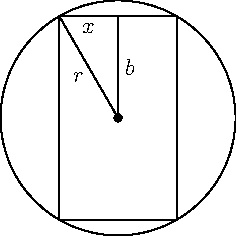
\includegraphics{opg7}\quad
	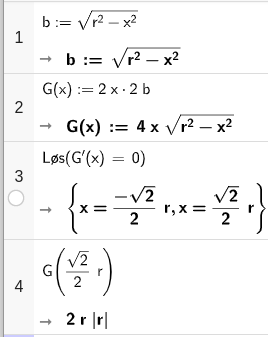
\includegraphics[scale=0.5]{opg7a}
\end{figure}
\end{document}